\documentclass[a4paper]{article}
\usepackage{epsfig,amsmath,amsfonts,amssymb,setspace,multirow,textcomp}
\usepackage[T1]{fontenc}
\usepackage{float}
\textheight 23cm \textwidth 18cm \hoffset= 0mm \voffset= 0cm
\topmargin -1cm \oddsidemargin -8mm \evensidemargin 0mm \columnsep = 4ex
% end of preamble

\begin{document}
\section*{\sc introduction}
\indent \indent Physical conditions in nebulae (planetary nebulae, large HII regions) 
are usually obtained using so called diagnostic method, that allows to obtain average 
the electron temperature $T_e$ and density $N_e$ from different emission line intensities ratios 
(see, f.e., DIAGN method \cite{DIAGN}). However, in case of diagnostic methods 
obtained $T_e$ and $N_e$ are constant within investigated ionization zone. 
For detailed analysis of the ionization structure of nebular environment 
the transfer of the ionizing radiation taking into account all elementary processes
in nebular plasmas important for such transfer should be calculated.
Such calculations are performed during PhM of nebular environment.

In case of nebulae with compact ionization source (f.e star, compact stars cluster, etc) 
radiation can be separated into two components:
\begin{enumerate}
\item Direct component, comming from ionizing source;
\item Diffuse component, originating from nebular gas.
\end{enumerate}

While transfer of the direct component of the ionizing radiation can be easy calculated
(because of no source terms), the diffuse radiation transfer calculation 
is a very time consuming even for modern supercomputers, 
since it requires iterative process of ionizing radiation flux integration over volume 
in each elementary cell of nebula environment. For time economy purpouses approximate methods 
of diffuse radiation calculation are frequently used. The most popular are {\b OTS} approximation, 
that assumes that ionizing radiation is consumed into the same volume where it whas emited, 
and {\b Outward Only} approximation, that assumes that ionizing radiation is propogated 
in radial direction, from ionizing source to outer surface of object. However, OTS method 
is good only in case of optically thick objects. Outward only approximation is more precise, 
however it can be inacurate in case of objects with complicated morphology. 
For example, dense clumps can cause the origination of shaded regions behind of them.
Non-radial DIR can play main role in formation of the ionization structure in these shaded
regions.

To avoid usage of approximate methods for DIR calculation and reduce time, 
required for PhM we developed {\b DiffRay3D}) software, that allows to integrate
radiation fluxes using 2D or 3D emissivity maps, and, as result, to implement 
method for detailed diffuse radiation calculation, described in \cite{JPS2016}
and displayed in Figure \ref{our_approach}.

\begin{figure}[!h]
\centering
\begin{minipage}[t]{.45\linewidth}
\centering
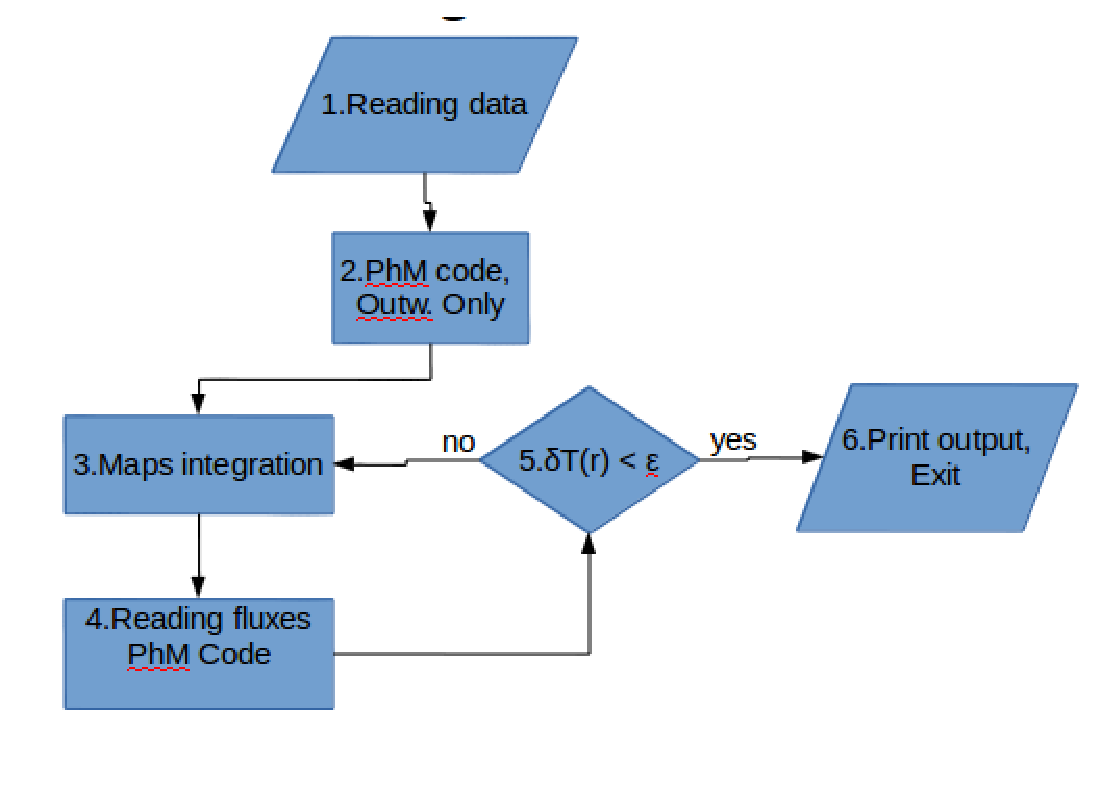
\epsfig{file = our_algo.eps,width = .85\linewidth}
\caption{Our approach algorithm}\label{our_approach}
\end{minipage}
\hfill
\end{figure}

\indent1 - Reading data, such as required precision, maximum iterations, etc.\\
\indent2 - Running PhM code in Outward Only mode, generating and saving emissivity and opacity maps.\\
\indent3 - Running integration procedure using previously generated maps.\\
\indent4 - Running PhM code, using fluxes, obtained after step 3. Generating and saving new emissivity and opacity maps.\\
\indent5 - Check difference between electron temperatures obtained from current iteration and the previous one. Once difference is greater than is required by precision, pointed in 1, then returning to step 3.\\
\indent6 - Printing fluxes and ionization structure, obtained from PhM on last iteration.\\


\section{DiffRay3D. General algorithm and limitations}

Current DiffRay3D version provides tools for radiation fluxes integration 
using 2D maps over 3D volume (3D maps support will be implemented in next code
versions). Nebula is divided onto 80 sectors (20 per quoter, assuming cylinder 
symethry and physical conditions in each quoter are the same). Each sector divided 
onto slabs. Shell structure is defined from input emissivity/opacity maps.

General code algorithm is displayed below:

\begin{figure}
\begin{minipage}[t]{.45\linewidth}
\centering
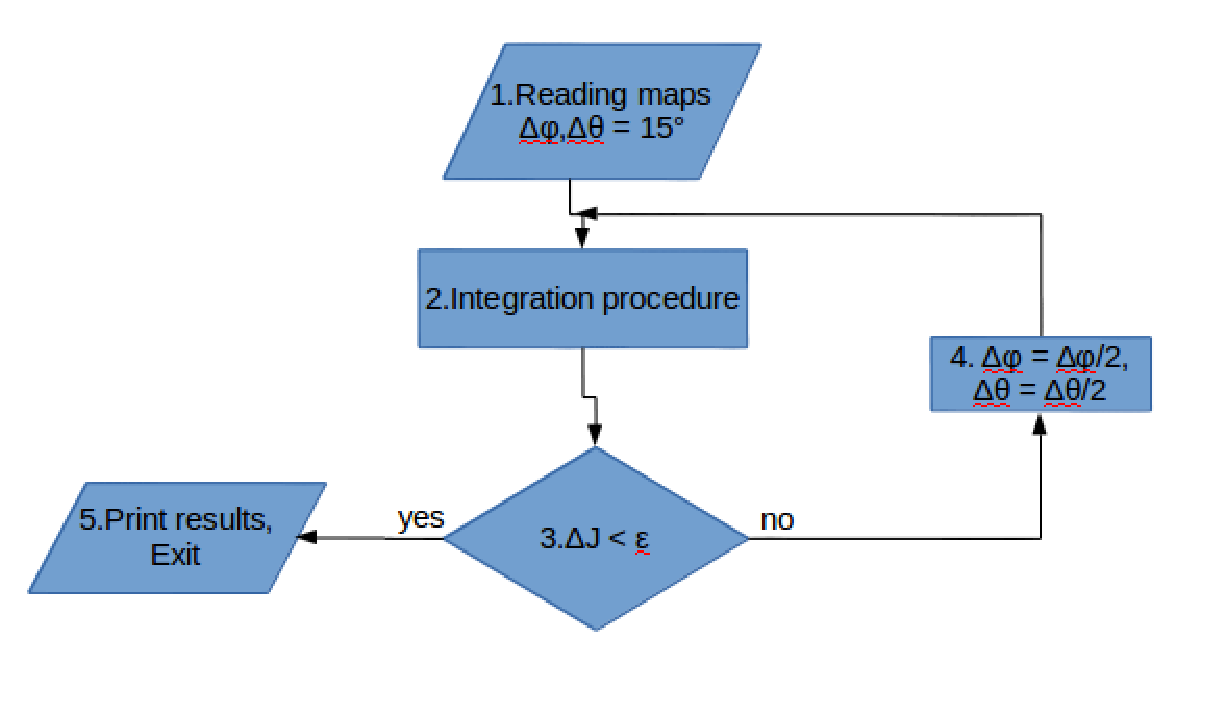
\epsfig{file = diffray_algo.eps,width = .85\linewidth}
\caption{DiffRay algorithm}\label{diffray_algo}
\end{minipage}
\end{figure}


For diffuse radiation fluxes integration procedure implementation DiffRay code was developed. The algorithm of code is given on figure \ref{diffray_algo}.\\
\indent1 - Setting up initial integration steps for angles, reading emissivity and opacity maps, that should be integrated.\\
\indent2 - Integration of diffuse radiation fluxes for each elementary volume of nebula environment\\
\indent3 - Comparing if difference between fluxes, obtained on current iteration and previous one. If it fits required precision, exit to 5. Elsewise, decreasing integration step (4), and returning to 2.\\
\indent5 - Print fluxes in format, that can be readen by PhM code. Exit.\\

\section{How to launch code}

To run code, you need working compiled code version, and valid object data with 
commands file provided.

\subsection{Code compilation}
1. Download code archive.\\
2. Unzip files in any folder you wish. DiffRay3D can be started into any folder, 
the only demand is code should have enough permissions for create/delete folders 
and files.\\
3. Once unzipped, go to "source/v*.*.*/" folder, and run MakeFile.all. This should
create DiffRay3D.exe executable into instalation root folder.\\

\section{Input data format}
To work correctly, code should have information about objects geometry, emissivity and opacity maps,
so on. This information is readen from data folder. In general, filename looks like:

Emis\_Lines\_SectorNo{\bf Sector number}\_Age{\bf Object age}Myr.dat

Here Sector number is number of represented by file sector
Age can be used as any identifier for model data set. (F.E. once you have maps for several models,
you can enumarate them, and use this numeration in age field.

Complete list of supported data files and their format can be found in next subsections.

\subsection{Continuum Mesh}
{\bf Continuum\{SectorNo\}\_Last\_Age10.00Myr.dat} - file with continuum energy mesh structure.
Each row should contain into first column continuum cell energy in Rydbergs. 
File is required. The structure of file is following:
\begin{table}[H]
\begin{tabular}{ll}
cell 1 energy & ... \\
cell 2 energy & ... \\
cell 3 energy & ... \\
cell 4 energy & ... \\
... & ... \\
\end{tabular}
\end{table}
Continuum cell energy should be represended in Rydberg units. File can contain arbitrary amount of columns, but only first one is used,
while the rest ones will be ignored.
If you want to change reading behavour, see {\it CContinuum::readMesh} method in "continuum.cpp" file.

\subsection{Continuum emissivities map}
{\bf Emis\_Cont\_SectorNo\{SectorNo\}\_Age10.00Myr.dat} - file with continuum emissivity data. Each row
corresponds to sector slab. First row has only one value - inner radius. Next rows contain slab outer radius in first column, 
and net volume emissivity values for each energy cell in corresponding slab in following columns. File is required. Note, that amount of columns in this file should
be equal to amount of rows in {\bf Continuum1\_Last\_Age10.00Myr.dat} + 1 column for radius.
The structure is following:
\begin{table}[H]
    \begin{tabular}{lll}
        inner radius & & \\
        Radius 1 & emissivity & ... \\
        Radius 2 & emissivity & ... \\
        Radius 3 & emissivity & ... \\
        ... & ... & ... \\
    \end{tabular}
\end{table}
Slab radius should be specified in centimeters. Emissivities are in $erg \cdot cm^-3 \cdot sec^-1$).
If you want to change reading behavour, see {\it CContinuum::readEmissivity} method in "continuum.cpp" file.

\subsection{Continuum opacities map}
{\bf Opac\_Cont\_SectorNo\{SectorNo\}\_Age10.00Myr.dat} - file with opacity data for each continuum cell. Each row
corresponds to sector slab. First row has only one value - inner radius. Next rows contain slab outer radius in first column, 
and opacity values for each energy cell in following columns. Used both for continuum and lines optical depth calculation. 
File is required.
The structure is following:
\begin{table}[H]
    \begin{tabular}{lll}
        inner radius & & \\
        Radius 1 & emissivity & ... \\
        Radius 2 & emissivity & ... \\
        Radius 3 & emissivity & ... \\
        ... & ... & ... \\
    \end{tabular}
\end{table}
Slab radius should be specified in centimeters. Opacities are in $cm^-1$.
If you want to change reading behavour, see {\it CContinuum::readOpacity} method in "continuum.cpp" file.

\subsection{Lines Emissivity}
\label{dataLines}
{\bf Emis\_Lines\_SectorNo\{SectorNo\}\_Age10.00Myr.dat} - file with lines emissivity data. Each row
corresponds to sector slab. First 2 rows has heading, according to standart Cloudy 
"punch line emisivity" command, \cite{Cloudy}. Next rows contain slab outer radius in first column, 
and emissivity values for each emission line in following columns. File is required.
The structure is following:
\begin{table}[H]
    \begin{tabular}{llll}
        heading & & & \\
        heading & line name & line name & ...\\
        Radius 1 & emissivity & emissivity & ... \\
        Radius 2 & emissivity & emissivity & ... \\
        Radius 3 & emissivity & emissivity & ... \\
        ... & ... & ... & ... \\
    \end{tabular}
\end{table}
Slab radius should be specified in centimeters. Emissivities are in $erg \cdot cm^-3 \cdot sec^-1$).
If you want to change reading behavour, see {\it CLines::readLines} method in "lines.cpp" file.

    {\bf Important Note: } you can specify only lines defined in known lines database. To check if line exists
    and supported you can search {\it data/database/line\_ch.data} for line label or in {\it data/database/line\_en.data}.
    If you can't find desired line - you can add it by editing these files. It's highly recommended, however, to add any new lines
    in the end of files. Also, if you edit these files - don't forget to copy them before you update DiffRay. Otherwise.
    data you changed will be overwriten.

\subsection{Chemical Abundance}
\label{dataAbund}
{\bf Abund\{SectorNo\}\_Age10.00Myr.dat} - file with elemental aundances data. Each row
corresponds to sector slab. First row should have valid column headings
with element names, provided as first 4 symbols of full name. 
(\#Depth		H	HELI	LITH	BERY..., Garry Ferlands Cloudy output 
format, see \cite{Cloudy}).
Next rows contain slab outer radius in first column, 
and elemental abundances for each element in following columns. File is not required.
The structure is following:
\begin{table}[H]
    \begin{tabular}{llll}
        Heading & Element 1 label & Element 2 label & ...\\
        Radius 1 & Abundance Value & Abundance Value & ... \\
        Radius 2 & Abundance Value & Abundance Value & ... \\
        Radius 3 & Abundance Value & Abundance Value & ... \\
        ... & ... & ... & ... \\
    \end{tabular}
\end{table}
Slab radius should be specified in centimeters. Abundances are represented as $log_10(Element Particle Count / Total Particle Count)$.
If you want to change reading behavour, see {\it Abund::getElementList} method in "abund.cpp" file.

\subsection{Physical Conditions Overview File}
\label{dataOverview}
{\bf Overview\{SectorNo\}\_Age10.00Myr.dat} - file with additional data about physical conditions. Each row
corresponds to sector slab. First row is heading.
(\#Depth		Te	Htot hden eden ..., Garry Ferlands Cloudy output of {\it punch overview}
format, see \cite{Cloudy}).
Next rows contain slab outer radius in first column,
and corresponding values, like electron temperature, electron density and so on.
The structure is following:
\begin{table}[H]
    \begin{tabular}{llllll}
        Heading & & & & & \\
        Radius 1 & Electron Temperature & Heating Rate & Density & Electron Density & ... \\
        Radius 2 & Electron Temperature & Heating Rate & Density & Electron Density & ... \\
        Radius 3 & Electron Temperature & Heating Rate & Density & Electron Density & ... \\
        ... & ... & ... & ... & ... & ... \\
    \end{tabular}
\end{table}
Slab radius should be specified in centimeters. Physical values are represented mostly in log scale.
If you want to change reading behavour, columns order and so on, see {\it Physics::readPhysics} method in "physics.cpp" file.


\section{Commands file}

Once you have compiled code and prepared data files, you should write some 
instructions for how and what code should calculated. These instructions are 
contained into commands.ini file into instalation root directory. 

An example is distributed with code source. \\

\subsection{IO settings}
{\it print directory "path to your output folder, relative to instalation root directory"} - set path to folder where output files will be located\\
{\it input directory "path to input data files folder, relative to instalation root directory"} - set path to folder with input data\\

{\bf Example:}\\
print directory result/ngc/ism0/140\\
input directory data/ngc1569nograin\\
Please, note that paths should be provided without quotes!\\

\subsection{Geometry and distance}
Commands that control object position in space.
{\bf Distance}\\
{\it distance log10\_dist units}.\\

{\bf Example:}\\
distance 19.87 km \\
(Distance to object is adopted of $10^{19.87}$ kilometers.
Supported units are meters, kilometers, centimeters.

{\bf Object}\\
{\it object phi x} , x - objects azimuthal rotation angle relating to observer sight ray in radians;\\
{\it object theta x} , x - objects vertical rotation angle relating to observer sight ray in radians;\\
{\it object age x}, x - object age, or another models bundle identifier; Currently doesn't have any impact on any calculations\\

{\bf Example:}\\
object phi 0.76\\
object theta 0.21\\
object age 50\\

\subsection{Calculation and integration options}
{\bf Integration}\\
{\it integration maxiterations x}, x - maximum code iterations. This option is useful to prevent code
falling into endless loop when trying to converge.\\
{\it integration precision x}, x - acceptable convergence between iterations, 0.01 - 1\%. \\
{\it integration mode outw} - switches code to Outward Only mode, is good thing for tests.\\
{\it integration predictive on} - turns on additional iteration, that runs before main process of splitting object onto spatial angles and solving
radiative transfer for those. This step tries to predict how much fluxes are changed along different sightlines within some angular sector
to determine desired initial angular integration step. It is recommended to turn on only in case of object with complex geometry and/or
significant spacial inhomogenities.

{\bf Example:}\\
integration precision 0.005\\
integration maxiterations 12\\
integration predictive off\\

{\bf Calculation}\\
calculation \{scope\} on/off - controls what kind of calculations DiffRay should perform. \\
{\it calculation opacity on/off} - turn on/off opacity calculation (turning this off assumes that environment is very opticlly thin for all
quantum) \\
{\it calculation continuum on/off} - turn on/off radiative transfer for continuum. Turning off will make DiffRay to calculate only line fluxes \\
{\it calculation abundance on/off} - turn on/off calculation of weighted elemental abundances within volume cut by aperture/along observer sightline. Once you turn this on,
abundance data files are required (See \ref{dataAbund} for details). \\
{\it calculation overview on/off} - turn on/off calculation of average electron temperature and density within volume cut by aperture/along observer sightline. Once you turn this on,
abundance data files are required (See \ref{dataOverview} for details). \\

\subsection{Isophotes}
isophote \{line | ratio\} \{line label\} - prints map of fluxes for selected line within square cut by aperture. \\
Can be useful to visualize spatial distribution of modeling volume brightness in specific emission lines. \\
{\it isophote line 'line label'} - prints map of absolute fluxes for selected line \\
{\it isophote ratio 'line label'} - prints map of relative fluxes for selected line ($F(selected line)/F(H_{\beta})$)) \\


\subsection{Aperture}

{\it aperture phi theta w h} - Adds aperture to list of apertures to be calculated.
Here phi - azimuthal aperture position, theta - vertical position relative to ray
from observer to center of object. w, h - aperture width and height. All values
should be provided into radians.\\

{\bf Example:}\\
apperture add 0 0 0.000014537 0.000014537\\
apperture add 0.000464 0.0000139 0.000014537 0.000014537\\
apperture add -0.000271 -0.0000102 0.000014537 0.000014537\\
In this example code will run calculations for 3 apertures, and put results to 
app\{N\} folder. N is aperture number here. Aperture folders are created automatically
into directory, specified with output command.

\section{Output}
Output files will be stored in the output directory specified in the corresponding commands file command.

\subsection{Emission Lines Results}
{\bf linesarr.dat} - a file containing fluxes for each line specified in the line emissivities input file (see \ref{dataLines}).
Each row contains four columns: line label, Flux at observer ($\mathrm{erg} \cdot \mathrm{cm}^{-2} \cdot \mathrm{s}^{-1}$), Luminosity ($\log_{10}(\mathrm{erg} \cdot \mathrm{s}^{-1})$),
and relative flux ($F(\text{line})/F(H_{\beta})$).\\
{\bf llum.dat} - an alternative representation of line luminosities. The file contains only two rows: a header, and luminosities for each line specified in the line emissivities input file (see \ref{dataLines}).
Luminosity is printed as ($\log_{10}(\mathrm{erg} \cdot \mathrm{s}^{-1})$). \\
{\bf lifr.dat} - an alternative representation of line fluxes. The file contains only two rows: a header, and fluxes for each line specified in the line emissivities input file (see \ref{dataLines}).
Fluxes are printed as ($\mathrm{erg} \cdot \mathrm{cm}^{-2} \cdot \mathrm{s}^{-1}$).

\subsection{Continuum Output}
{\bf contarr.dat} - contains continuum fluxes at different photon energies. It contains three columns:
1 - Photon energy, 2 - amount of quanta of attenuated incident continuum ($\mathrm{cm}^{-2} \cdot \mathrm{s}^{-1}$), 3 - amount of quanta of diffuse continuum ($\mathrm{cm}^{-2} \cdot \mathrm{s}^{-1}$).\\

More output files with additional formats are planned for the future.

\subsection{Chemical Abundances}
{\bf abmass.txt} - contains the abundances of elements within a volume cut by an aperture within the object, weighted by mass.
It has two rows: a heading and a list of weighted abundances ($12 - \log_{10}(n(\text{element})/n(H))$). \\

{\bf abemso.txt} - contains the abundances of elements within a volume cut by an aperture within the object, weighted by oxygen
lines emissivity ($e(O3  5007\text{\AA}) + e(O3  4363\text{\AA}) + e(O3  4959\text{\AA}) + e(O2  3726\text{\AA}) + e(O2  3729\text{\AA})$).
It has two rows: a heading and a list of weighted abundances ($12 - \log_{10}(n(\text{element})/n(H))$).

\subsection{Isophotes}

{\bf isophote\_\{index\}.dat} - file containing 2D data for drawing flux maps.
The 1st and 2nd columns represent spatial angles, and the 3rd column lists the fluxes calculated from the direction determined by these spatial angles.

When 'isophote' commands are present, gnuplot scripts for visualization are generated and located in the "plots"
folder within your output directory.


\begin{thebibliography}{3}
{\small
\bibitem{DIAGN} Golovaty V.\,V., Dmiterko V.\,I., Mal'kov Yu.\,F., \& Rokach O.\,V. 1993, Astronomical Report, Vol. 37, Issue 4, pp. 346-354
\bibitem{JPS2016} O. S. Buhajenko, B. Ya. Melekh 2016, `METHOD FOR DETAILED CALCULATION OF THE DIFFUSE IONIZING RADIATION IN NEBULAR ENVIRONMENTS`, Ivan Franko National University of Lviv, 4901 (13 p.) 
\bibitem{Cloudy} Ferland G.J. 1999, `Hazy, a Brief Introduction to Cloudy 94`, University of Kentucky, Physics Department Internal Report; \texttt{http://www.nublado.org}
}
\end{thebibliography}
\end{document}
